\section{An extended example}
To get a better feel for how a feedback control system works in practice, we will discuss a simple but interesting application of feedback control that uses the theory covered in the previous sections. In this section we show an imperative reference implementation. In the next chapter we will continue to use and refactor this application as we come up with an API for constructing and executing feedback systems. The application at hand is a port from the original implementation by Nikita Leshenko in Javascript, CSS and HTML \cite{nikital-balltracker}. We will however use Scala as our programming language and JavaFx for drawing the graphics on the screen.

The application consists of a flat surface on which a ball can move around. The goal is to move the ball from its initial position to the position on the surface that the user clicks on with the mouse. \autoref{fig:balltracker-initial} shows the ball in its initial state when the application starts. When the user clicks on the screen, the ball starts moving to that position as shown by \autoref{fig:balltracker-moving}. Besides the background and the ball, also the desired position, a dashed line between the ball and the desired position, the acceleration in both the $x$ and $y$ directions and a trail of previous positions are drawn (which are fading away over time). After some time the ball is at its desired position and waits there for a new position to navigate to (\autoref{fig:balltracker-reached}). Notice that the desired position can also be updated while the ball is still moving, in which case it moves to the new and discards the old destination.

In order to allow the ball to move in a natural way, we remind the reader of some basic equations from physics that describe the one dimensional motion of an object as a function of time (\autoref{eq:motion}). Here $x_t$, $v_t$ and $a_t$ are the ball's position, velocity and acceleration at time $t$ respectively. For two-dimensional motion we can combine two sets of these equations for both dimensions.

\begin{subequations}
	\begin{equation}
		x_t = x_{t - 1} + v_t \cdot \Delta t
	\end{equation}
	\begin{equation}
		v_t = v_{t - 1} + a_t \cdot \Delta t
	\end{equation}
	\label{eq:motion}
\end{subequations}

\begin{figure}
	\centering
	\begin{subfigure}[b]{0.80\linewidth}
		
\includegraphics[trim = 0mm 110mm 0mm 0mm, clip, width=\linewidth]{figures/BallTracker-initial.png}
		\caption{Initial}
		\label{fig:balltracker-initial}
	\end{subfigure}
	
	\begin{subfigure}[b]{0.80\linewidth}
		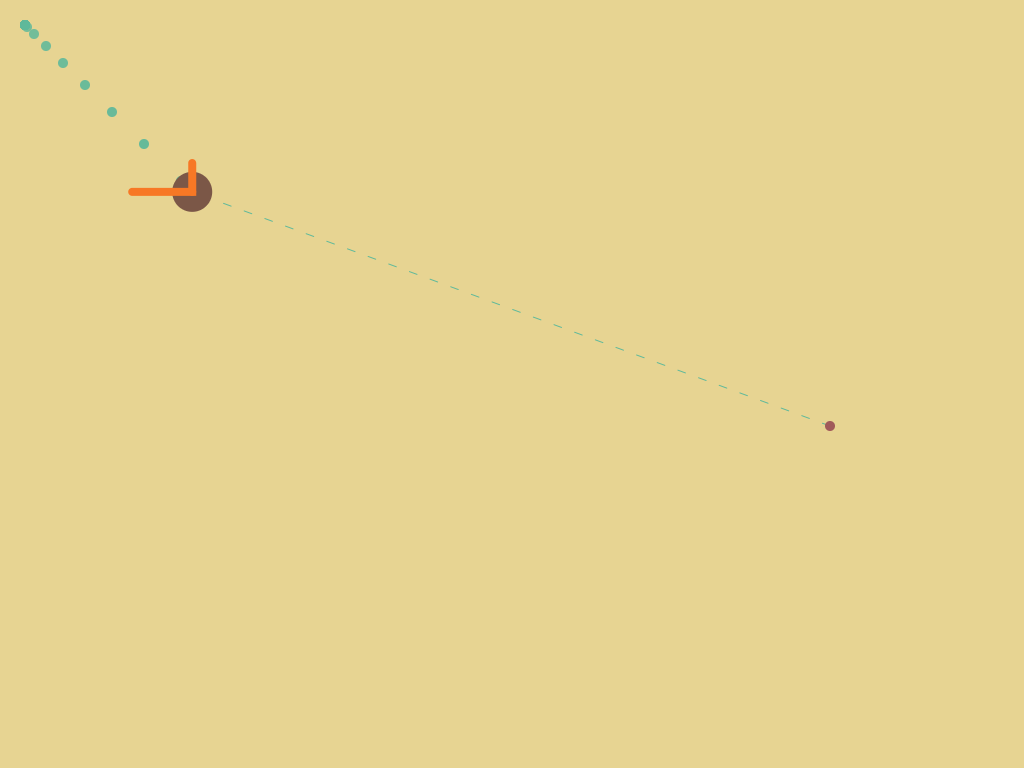
\includegraphics[trim = 0mm 110mm 0mm 0mm, clip, width=\linewidth]{figures/BallTracker-moving.png}
		\caption{Moving to desired position}
		\label{fig:balltracker-moving}
	\end{subfigure}
	
	\begin{subfigure}[b]{0.80\linewidth}
		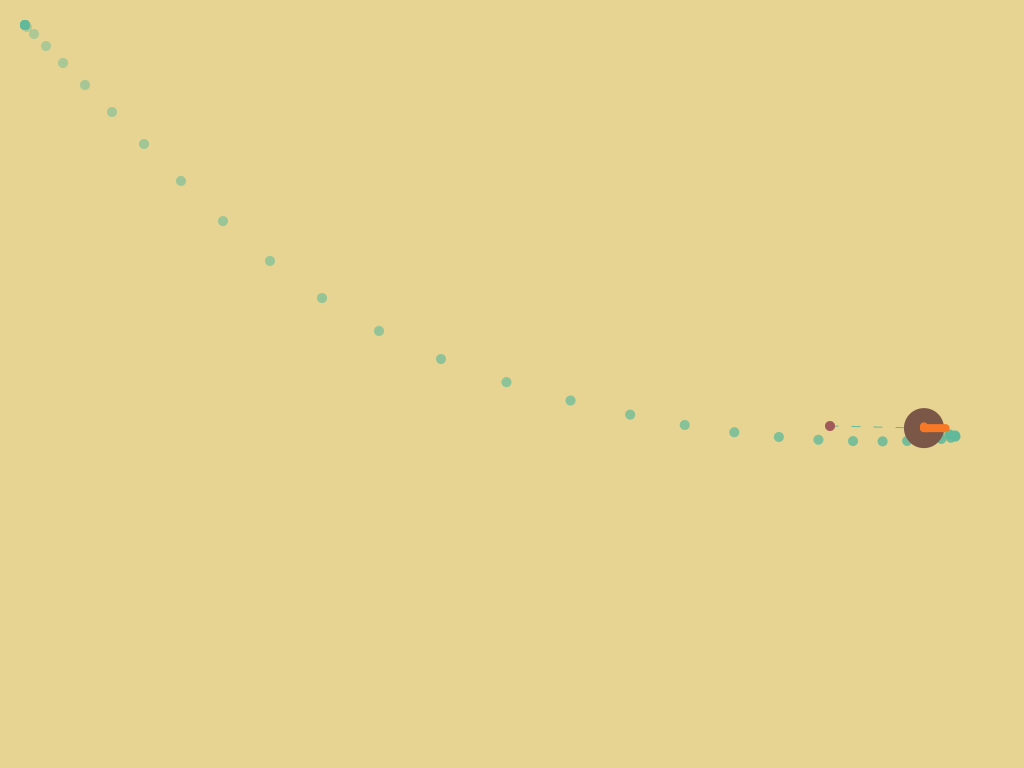
\includegraphics[trim = 0mm 110mm 0mm 0mm, clip, width=\linewidth]{figures/BallTracker-overshooting.png}
		\caption{Moving to desired position}
		\label{fig:balltracker-moving}
	\end{subfigure}
	
	\begin{subfigure}[b]{0.80\linewidth}
		
\includegraphics[trim = 0mm 110mm 0mm 0mm, clip, width=\linewidth]{figures/BallTracker-desired.png}
		\caption{Reached desired position}
		\label{fig:balltracker-reached}
	\end{subfigure}
	\caption{Ball tracker}
	\label{fig:balltracker}
\end{figure}

We define these required pieces of physics in \autoref{lst:ball-physics}. We first define a \code{Position}, \code{Velocity} and \code{Acceleration} as tuples of \code{Double} as well as mathematical operations on the tuple type. The \code{Ball} class describes the current state of the ball having a position, velocity and acceleration. A second constructor (\code{apply}) defines the initial position with no acceleration or velocity. The method \code{accelerate} on this class takes a new acceleration and calculates the new state for the ball according to \autoref{eq:motion}. Notice that we discard the $\Delta t$ term as this is always equal to 1. To keep track of the ball's previous positions we define a type \code{History}, being a queue of \code{Position}s.

\begin{minipage}{\linewidth}
\begin{lstlisting}[style=ScalaStyle, caption={Ball motion physics}, label={lst:ball-physics}]
type Position $=$ (Double, Double)
type Velocity $=$ (Double, Double)
type Acceleration $=$ (Double, Double)
type History $=$ mutable.Queue[Position]

implicit class Tuple2Math[X: Numeric, Y: Numeric](val src: (X, Y)) {
  import Numeric.Implicits._
  def +(other: (X, Y)) $=$ (src._1 + other._1, src._2 + other._2)
  def -(other: (X, Y)) $=$ (src._1 - other._1, src._2 - other._2)
  def *[Z](scalar: Double) $=$ (src._1.toDouble * scalar, src._2.toDouble * scalar)
  def map[Z](f: X $\Rightarrow$ Z)(implicit ev: Y $=:=$ X): (Z, Z) $=$ {
    ((x: X, y: Y) $\Rightarrow$ (f(x), f.compose(ev)(y))).tupled(src)
  }
}

case class Ball(acc: Acceleration, vel: Velocity, pos: Position) {
  def accelerate(newAcc: Acceleration): Ball $=$ {
    Ball(newAcc, vel + newAcc, pos + vel + newAcc)
  }
}
object Ball {
  def apply(radius: Double): Ball $=$ {
    Ball((0.0, 0.0), (0.0, 0.0), (radius, radius))
  }
}
\end{lstlisting}
\end{minipage}

\todo{text here}

%\begin{minipage}{\linewidth}
\begin{lstlisting}[style=ScalaStyle, caption={Ball drawing}, label={lst:ball-drawing}]
object Draw {
  def draw(pos: Position, setpoint: Position, acc: Acceleration, history: History)(implicit gc: GraphicsContext) $=$ {
    drawBackground
    drawHistory(history)
    drawLine(pos, setpoint)
    drawSetpoint(setpoint)
    drawBall(pos)
    drawVectors(pos, acc)
  }

  def drawBackground(implicit gc: GraphicsContext) $=$ {
    gc.setFill(Color.rgb(231, 212, 146))
    gc.fillRect(0, 0, width, height)
  }

  def drawBall(point: Position)(implicit gc: GraphicsContext) $=$ {
    val (x, y) $=$ point
    val diameter $=$ 2 * ballRadius

    gc.setFill(Color.rgb(123, 87, 71))
    gc.fillOval(x - ballRadius, y - ballRadius, diameter, diameter)
  }

  def drawSetpoint(setpoint: Position)(implicit gc: GraphicsContext) $=$ {
    val (x, y) $=$ setpoint
    val radius $=$ ballRadius / 4
    val diameter $=$ radius * 2

    gc.setFill(Color.rgb(161, 90, 90))
    gc.fillOval(x - radius, y - radius, diameter, diameter)
  }

  def drawLine(ball: Position, setpoint: Position)(implicit gc: GraphicsContext) $=$ {
    val (bx, by) $=$ ball
    val (sx, sy) $=$ setpoint

    gc.setStroke(Color.rgb(96, 185, 154))
    gc.setLineWidth(1.0)
    gc.setLineDashes(8.0, 14.0)

    gc.beginPath()
    gc.moveTo(sx, sy)
    gc.lineTo(bx, by)
    gc.stroke()
    gc.setLineDashes()
  }

  def drawVectors(pos: Position, acc: Acceleration)(implicit gc: GraphicsContext) $=$ {
    val (px, py) $=$ pos
    val (ax, ay) $=$ acc

    gc.setStroke(Color.rgb(247, 120, 37))
    gc.setLineWidth(8)
    gc.setLineCap(StrokeLineCap.ROUND)

    gc.beginPath()
    gc.moveTo(px, py)
    gc.lineTo(px - ax * 300, py)
    gc.stroke()

    gc.beginPath()
    gc.lineTo(px, py)
    gc.lineTo(px, py - ay * 300)
    gc.stroke()
  }

  def drawHistory(history: History)(implicit gc: GraphicsContext) $=$ {
    history.synchronized {
      history.zipWithIndex.foreach(item $\Rightarrow$ {
        val (pos, index) $=$ item
        val (x, y) $=$ pos
        val size $=$ history.size
        val alpha $=$ (index: Double) / size

        gc.setFill(Color.rgb(96, 185, 154, alpha))
        gc.fillOval(x, y, 10, 10)
      })
    }
  }
}
\end{lstlisting}
%\end{minipage}